\documentclass[conference]{IEEEtran}
\IEEEoverridecommandlockouts

\usepackage{cite}
\usepackage{amsmath,amssymb,amsfonts}
\usepackage{graphicx}
\usepackage{textcomp}
\usepackage{xcolor}
\usepackage{booktabs}
\usepackage{multirow}
\usepackage{tikz}
\usetikzlibrary{arrows.meta,positioning}
\usepackage[T1]{fontenc}
\usepackage[utf8]{inputenc}

\graphicspath{{res/}}

\def\BibTeX{{\rm B\kern-.05em{\sc i\kern-.025em b}\kern-.08em
    T\kern-.1667em\lower.7ex\hbox{E}\kern-.125emX}}

\begin{document}

\title{Federated Learning Decentralizzato Peer-to-Peer con Protocollo Gossip su FEMNIST}

\author{
\IEEEauthorblockN{Flavio Di Palma, Giordano Spirito}
\IEEEauthorblockA{
Corso di Laurea Magistrale in Ingegneria Informatica \\
Università degli Studi di Roma ``Tor Vergata'' \\
Roma, Italia
}
}

\maketitle

\begin{abstract}
Questo lavoro presenta la progettazione e la valutazione sperimentale di un
sistema di Federated Learning decentralizzato con protocollo di comunicazione push
one-hop a fanout fisso. Il sistema è applicato al
riconoscimento di caratteri manoscritti sul dataset non-i.i.d.\ FEMNIST del
progetto LEAF. A differenza del FedAvg centralizzato, nessun nodo
agisce da aggregatore per l'intera durata dell'addestramento: ciascun worker
alterna fasi di training locale e di aggregazione dei pesi ricevuti
dai vicini, mentre un componente centralizzato leggero è impiegato solo per
la service discovery. Il sistema è stato valutato con 16 configurazioni
sperimentali (8 in esecuzione locale, 8 su istanze AWS EC2), variando il numero
di client (3, 5, 8), il fanout di comunicazione e il
numero di passi locali tra due round di comunicazione. I risultati mostrano
un'accuratezza di validazione tra l'87\% e il 91\%, un costo di comunicazione
per round di circa 6,8\,MB per messaggio e una netta separazione tra il costo
del training locale e quello della fase di comunicazione, anche su rete reale.
\end{abstract}

\section{Introduzione}
\label{sec:introduction}

Il Federated Learning permette a un insieme di nodi client, ciascuno in
possesso di un dataset locale privato, di addestrare collaborativamente un
modello condiviso senza scambiare i dati grezzi. Nella formulazione centralizzata,
un server raccoglie i pesi locali
di ogni client, li aggrega secondo un particolare algoritmo e ridistribuisce il modello aggiornato: il server è
un single point of failure, la sua banda è un collo di bottiglia che cresce
con il numero di client, e ogni round richiede una sincronizzazione globale
al passo del client più lento.

Il presente lavoro affronta questi limiti progettando un sistema di FL
\emph{decentralizzato}: i pesi vengono scambiati tra i client tramite un
protocollo di comunicazione peer-to-peer a push one-hop e fanout fisso, in
cui ciascun client invia periodicamente i propri pesi a un sottoinsieme di
vicini scelti casualmente, e vengono aggregati localmente da chi li riceve
tramite FedAvg. Un componente centralizzato, il discovery server,
resta limitato esclusivamente alla registrazione e alla scoperta reciproca dei
client.

\section{Contesto}
\label{sec:background}

\subsection{FedAvg}
FedAvg aggiorna il modello globale come media dei
pesi locali, pesata per il numero di campioni di ciascun client:
\begin{equation}
  w \leftarrow \sum_{i=1}^{K} \frac{n_i}{n} w_i, \qquad n = \sum_{i=1}^{K} n_i
  \label{eq:fedavg}
\end{equation}
dove $w_i$ e $n_i$ sono rispettivamente i pesi e il numero di campioni di
addestramento del client $i$. Sotto ipotesi di dati non-i.i.d., la velocità di
convergenza di FedAvg degrada con il grado di eterogeneità tra le
distribuzioni locali.

\subsection{DiLoCo e comunicazione sparsa}
DiLoCo~\cite{douillard2023diloco} riduce la frequenza di comunicazione
alternando $H$ passi di ottimizzazione locale (\emph{inner steps}) a un
singolo passo di sincronizzazione globale, eseguito da un \emph{outer
optimizer} con momentum mantenuto centralmente. Il sistema qui presentato
adotta la stessa idea di comunicazione sparsa a $H$ passi, ma non può
adottare l'outer optimizer di DiLoCo così com'è: quest'ultimo richiede uno
stato di momentum globale coerente per tutti i client, il che presuppone
un coordinatore centrale. Il sistema sostituisce
quindi la sincronizzazione globale periodica di DiLoCo con un'aggregazione
locale asincrona basata su un push one-hop a fanout fisso tra vicini,
descritta nella Sezione~\ref{sec:design} e motivata per contrasto con le
alternative del corso nella Sezione~\ref{sec:background}E.

\subsection{Dataset: LEAF e FEMNIST}
FEMNIST è un dataset di caratteri manoscritti (cifre e
lettere, 62 classi, immagini $28\times28$ in scala di grigi) partizionato per
scrittore: ogni scrittore produce una distribuzione di stili ed etichette
propria, rendendo il dataset naturalmente non-i.i.d.\ tra client quando ogni
partizione corrisponde a scrittori diversi. Nel sistema qui presentato ogni
client riceve dati di \emph{più} scrittori LEAF, per simulare
uno scenario realistico in cui un partecipante rappresenta un piccolo gruppo
di utenti piuttosto che un singolo individuo.

\subsection{Strategie alternative non implementate}
La letteratura propone diverse estensioni di FedAvg per mitigare
l'eterogeneità dei dati: FedProx~\cite{li2020fedprox}, SCAFFOLD~\cite{karimireddy2020scaffold},
FedBN~\cite{li2021fedbn}. Il sistema qui presentato implementa esclusivamente FedAvg,
scelto come strategia di riferimento più semplice da rendere verificabile in
un contesto decentralizzato puro. Non tutte le
alternative sono equivalenti dal punto di vista architetturale: FedProx
modifica solo la funzione di costo usata in Fase B (Sezione~\ref{sec:details}B)
e potrebbe essere adottata senza alcuna modifica al buffer di aggregazione o
al protocollo gRPC; SCAFFOLD richiederebbe di trasmettere anche variabili di
controllo oltre ai pesi, aumentando la dimensione dei messaggi ma senza
introdurre un aggregatore centrale.

\subsection{Scelta del protocollo di comunicazione}
Il corso di riferimento presenta tre famiglie di disseminazione a livello
applicativo su overlay non strutturato: \emph{flooding},
\emph{random walk} e \emph{gossip epidemico}, a sua volta nelle
varianti \emph{anti-entropy} e \emph{rumor mongering}. Il sistema qui
presentato usa invece un
\textbf{push one-hop a fanout fisso $k$ con grpc} (Sezione~\ref{sec:details}B, indicato
anche come \emph{k-push}); i vicini sono scelti casualmente a ogni round,
un modello neutro di una qualunque politica di selezione reale (prossimità
di rete, similarità dei dati locali se disponibile, o un altro stato osservabile del nodo). I confronti
che seguono si riferiscono alle scale testate in questo lavoro, $N\le8$ — il
tetto imposto da AWS Learner Lab (Sezione~\ref{sec:details}F), non un limite
intrinseco del protocollo.

\textbf{Perché non flooding.} Il motivo principale è il traffico: il numero
di trasmissioni cresce con il grado medio dei vicini e, soprattutto, con il
\emph{time-to-live} — ogni hop aggiuntivo moltiplica i messaggi per il
fattore di ramificazione della rete.Il
caso limite $k=N-1$ del nostro push one-hop è di fatto equivalente a un singolo round di flooding con
\emph{time-to-live}$=1$: ogni worker raggiunge direttamente tutti i peer
noti, senza bisogno di alcun inoltro successivo. La differenza pratica tra le
due soluzioni emerge solo a \emph{time-to-live}$>1$, cioè quando servirebbe
più di un hop per coprire l'intera rete. Su reti più grandi e sparse il traffico
crescerebbe in modo moltiplicativo a ogni hop: resta quindi la soluzione più
costosa delle tre a qualunque scala.

\textbf{Il push one-hop equivale a $N$ k-random-walk simultanei.} Il singolo hop di trasporto coincide di
fatto con il primo passo di un \emph{k-random-walk} con
\emph{time-to-live}$=1$. La differenza non è tanto il \emph{time-to-live} quanto la molteplicità delle origini: un
k-random-walk parte da \emph{un solo} nodo con una query da propagare; il
nostro sistema fa ripartire lo stesso meccanismo da \emph{ogni} worker, ogni
round, in parallelo.

\textbf{Gossip epidemico.} È un'alternativa legittima: il relay multi-hop propagherebbe gli
aggiornamenti più rapidamente e più fedelmente all'originale, un vantaggio
reale su reti molto più grandi di quelle testate, dove un $k$ fisso non
basterebbe più a coprire l'intera rete in pochi round. Il costo è il
traffico (requisito del progetto)— ogni hop di relay moltiplica i messaggi per il fattore di
ramificazione, mentre il push one-hop mantiene un costo per nodo
indipendente da $N$ — quindi un compromesso esplicito tra traffico e
qualità/freschezza dell'informazione, da valutare caso per caso. La nostra soluzione, essendo applicata ad un contesto
di machine learning federato con fed avg, comunque propoaga ragionevolmente nel tempo l'informazione a tutta la rete,
anche se hop è 1, in quanto i messaggi con i nuovi pesi hanno "memoria" anche dei vecchi aggiornamenti.
Infatti il guadagno del relay è inoltre già in parte attenuato dal
dominio applicativo: grazie a FedAvg, lo stato che un worker invia è già il
risultato di aggregazioni con i round precedenti, quindi la propagazione
multi-hop avviene comunque, implicitamente, nel tempo anziché nello spazio
del singolo round. Il relay porterebbe anche un
problema standard di deduplicazione — lo stesso messaggio potrebbe
raggiungere lo stesso worker da percorsi indipendenti nello stesso round —
comunque risolvibile. Un osservazione: quando il payload scambiato è l'intero stato di un modello e non un piccolo
messaggio, il costo di un relay multi-hop cresce con il fattore di
ramificazione a ogni hop, mentre l'aggregazione locale ottiene una
propagazione senza traffico aggiuntivo dedicato al solo inoltro. In definitiva, abbiamo preferito restare entro i
vincoli di traffico richiesti esplicitamente dalla traccia di progetto;
resta un'osservazione interessante da approfondire in futuro come si
comporterebbe il gossip epidemico in un contesto con molti più nodi, e come
si confronterebbe con la soluzione qui proposta.


\textbf{Verifica empirica.} Il grafo one-hop raggiunge comunque la
connettività completa alle scale qui testate: con $k=N-1$ ogni worker
contatta \emph{tutti} i propri peer a ogni round, il limite superiore
raggiungibile in un singolo hop. I risultati (Sezione~\ref{sec:results}A,
Sezione~\ref{sec:discussion}A) mostrano che questo da solo chiude la
maggior parte del divario osservato a fanout basso (+7--8 punti di
accuratezza global-test tra $k=1$ e $k=N-1$ a $N=8$, spread quasi dimezzato);
ma anche a $k=N-1$ lo spread non scende mai sotto il 14\%
(Sezione~\ref{sec:discussion}D). Poiché $k=N-1$ è già la copertura massima
raggiungibile in un hop, un relay multi-hop non avrebbe potuto ridurre
ulteriormente questo residuo: la causa più probabile non è la portata del
protocollo di comunicazione, ma l'assenza di un meccanismo esplicito di
correzione del client drift (FedProx, SCAFFOLD, Sezione~\ref{sec:background}D)
— una limitazione indipendente dalla scelta tra one-hop e multi-hop, discussa
in Sezione~\ref{sec:discussion}D.

\section{Solution Design}
\label{sec:design}

\subsection{Panoramica architetturale}
Il sistema è composto da $K$ nodi \emph{worker} paritari e da un
\emph{discovery server} leggero (Fig.~\ref{fig:architecture}). Ogni worker
esegue due thread indipendenti: un server gRPC che riceve i modelli inviati
dai vicini (Fase C di un altro worker) e li accumula in un buffer condiviso,
e un ciclo di training che, a ogni round, aggrega quanto ricevuto, esegue
addestramento locale e invia i propri pesi a un sottoinsieme di vicini.
Qualunque worker può avviare il proprio processo di training in autonomia,
leggendo iperparametri e riferimenti dei peer coinvolti da una configurazione
condivisa (\texttt{config.yaml}) e dal discovery server; non esiste un nodo
che comandi l'avvio degli altri. Questo soddisfa la decentralizzazione
dell'\emph{avvio} richiesta dalla traccia — nessun coordinatore privilegiato
è necessario. Il sistema resta però un job sincronizzato all'avvio, non un
servizio always-on: prima di iniziare il training, ogni worker attende
(Sezione~\ref{sec:details}A) che l'intera coorte di $K$ client configurati
sia online, con un timeout oltre il quale procede comunque con i peer
disponibili; un client non può quindi iniziare una nuova sessione in un
istante arbitrario senza un nuovo deployment, un limite condiviso con la
generalità dei job di training distribuito (analogamente a un job
SLURM/MPI) e discusso in Sezione~\ref{sec:conclusions} come possibile
estensione.

Il discovery server espone quattro sole operazioni REST
(\texttt{/register}, \texttt{/deregister}, \texttt{/peers}, \texttt{/health}),
mantiene in memoria una mappa \texttt{worker\_id~$\to$~indirizzo} e non
riceve, memorizza o media mai un peso del modello. Il suo unico compito
aggiuntivo è un \emph{watchdog} che forza la terminazione del cluster se un
worker non si deregistra correttamente entro un timeout — una funzione di
coordinamento della terminazione, non di training. Questo confina la
centralizzazione ai soli compiti di avvio/terminazione e identificazione dei
client, come richiesto dalla traccia. Il raggio d'azione di questo singolo
componente centralizzato è inoltre limitato nel tempo: la lista dei peer è
letta una sola volta all'avvio (Sezione~\ref{sec:details}C) e sia
\texttt{fetch\_peers} sia \texttt{deregister\_worker} degradano senza
propagare l'errore se il discovery server non risponde. Un guasto del
discovery server dopo l'avvio blocca quindi solo l'ingresso di nuovi client,
non il gossip già in corso tra quelli attivi, che continuano a operare sulla
propria cache locale.

\begin{figure}[t]
  \centering
  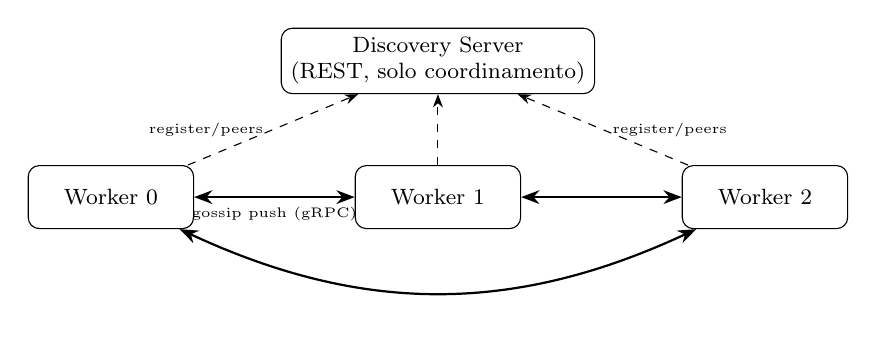
\begin{tikzpicture}[
      node distance=0.9cm and 1.1cm,
      box/.style={draw, rounded corners, minimum width=2.1cm, minimum height=0.8cm, align=center, font=\footnotesize},
      >=Stealth
    ]
    \node[box] (reg) {Discovery Server\\(REST, solo coordinamento)};
    \node[box, below left=of reg] (w0) {Worker 0};
    \node[box, below=of reg] (w1) {Worker 1};
    \node[box, below right=of reg] (w2) {Worker 2};

    \draw[dashed, ->] (w0) -- node[left, font=\tiny]{register/peers} (reg);
    \draw[dashed, ->] (w1) -- (reg);
    \draw[dashed, ->] (w2) -- node[right, font=\tiny]{register/peers} (reg);

    \draw[<->, thick] (w0) -- node[below, font=\tiny]{gossip push (gRPC)} (w1);
    \draw[<->, thick] (w1) -- (w2);
    \draw[<->, thick] (w0) to[bend right=25] (w2);
  \end{tikzpicture}
  \caption{Architettura logica: il discovery server gestisce solo la
  registrazione (linee tratteggiate REST); i modelli viaggiano esclusivamente
  peer-to-peer via gRPC (frecce continue). Il grafo tra worker è
  \emph{potenziale}, non fisso: a ogni round ciascun worker sceglie
  casualmente $k$ destinatari tra i peer disponibili, senza inoltro da parte
  di chi riceve (Sezione~\ref{sec:background}E).}
  \label{fig:architecture}
\end{figure}

\subsection{Aggregazione decentralizzata}
Ogni worker mantiene un buffer di aggregazione protetto da lock. Quando un
messaggio gossip arriva, il server gRPC non lo accoda: lo somma
immediatamente, pesato per il numero di campioni del mittente, a un
accumulatore già esistente (\emph{online aggregation}). Il costo in memoria e
in tempo di questa operazione è quindi $O(\text{dimensione del modello})$ e
non $O(K \cdot \text{dimensione del modello})$ come sarebbe mantenendo una
lista di tutti i modelli ricevuti. All'inizio del round successivo, il thread
di training applica FedAvg (Eq.~\ref{eq:fedavg}) tra il proprio modello e la
somma pesata accumulata, quindi svuota il buffer. In nessun momento un nodo
possiede o osserva i pesi di \emph{tutti} gli altri $K-1$ client
contemporaneamente: ciascun worker aggrega solo ciò che i suoi vicini gli
hanno inviato, realizzando un'aggregazione FedAvg genuinamente
peer-to-peer e priva di un aggregatore singolo per l'intera durata del
processo.

\subsection{Motivazione delle scelte protocollari}
La comunicazione tra worker usa gRPC su Protobuf anziché REST/JSON: la
serializzazione binaria di un \texttt{state\_dict} PyTorch produce un
messaggio 2--3$\times$ più compatto rispetto alla codifica testuale
equivalente, un risparmio non trascurabile quando ogni messaggio trasporta
l'intero modello (Sezione~\ref{sec:results}). La lista dei peer è letta dal
discovery server una sola volta, all'avvio (Sezione~\ref{sec:details}A), e
tenuta in una cache locale per l'intera durata del training: se il worker
la reinterrogasse a ogni round, il traffico verso il discovery server
crescerebbe linearmente con il numero di round anziché restare $O(1)$ per
l'intera run, vanificando in parte l'obiettivo di traffico ridotto che
motiva anche la scelta del k-push (Sezione~\ref{sec:background}E). La cache
viene aggiornata solo lazily, cioè non periodicamente ma esclusivamente
quando serve: ogni invio ha un timeout configurabile e, in caso di
fallimento, il worker interroga di nuovo il discovery server e ritenta una
sola volta con peer non ancora contattati in quel round — evitando sia
blocchi su nodi caduti sia un sovraccarico di richieste al discovery server
nei round in cui tutto funziona normalmente.

\subsection{Aderenza ai requisiti}
La Tabella~\ref{tab:requirements} riassume come ciascun requisito della
traccia (progetto ML e vincoli imposti per il corso di Sistemi Distribuiti e
Cloud Computing) sia stato affrontato.

\begin{table}[t]
  \centering
  \caption{Mappatura requisiti $\to$ soluzione adottata.}
  \label{tab:requirements}
  \footnotesize
  \begin{tabular}{p{2.3cm}p{5.3cm}}
    \toprule
    \textbf{Requisito} & \textbf{Come è soddisfatto} \\
    \midrule
    Team di 2 studenti & Progetto sviluppato da 2 autori; la modalità
      centralizzata con parameter server è opzionale solo per team da 3 e
      non è stata implementata. \\
    $K$ client, avvio autonomo & Ogni worker legge \texttt{config.yaml} e
      avvia il proprio ciclo di training senza comando esterno
      (Sez.~\ref{sec:design}A). \\
    Scelta della strategia di aggregazione & FedAvg selezionabile via
      \texttt{aggregation\_strategy} in configurazione; unica strategia
      implementata (Sez.~\ref{sec:background}D). \\
    Centralizzazione limitata al coordinamento & Discovery server: solo
      register/deregister/peers/health, mai pesi del modello
      (Sez.~\ref{sec:design}A). \\
    Aggregazione P2P, no aggregatore singolo & Aggregazione online nel
      buffer di ciascun worker, gossip $k$-push (Sez.~\ref{sec:design}B). \\
    LEAF, più utenti per client & FEMNIST partizionato per scrittore, blocchi
      di scrittori per worker (Sez.~\ref{sec:details}A). \\
    Scalabilità: accuracy e tempi vs $N$ & $N \in \{3,5,8\}$ testati sia in
      locale sia su AWS multi-istanza (Sez.~\ref{sec:results}). \\
    Efficienza di comunicazione & Dimensione messaggio, traffico stimato e
      tempo di Fase C misurati separatamente dal training
      (Sez.~\ref{sec:results}). \\
    Fault tolerance (opzionale) & Crash/drop injection, timeout, retry,
      staleness check (Sez.~\ref{sec:details}C). \\
    \bottomrule
  \end{tabular}
\end{table}

\section{Dettagli implementativi}
\label{sec:details}

\subsection{Partizionamento non-i.i.d.\ del dataset}
Il dataset FEMNIST scaricato in formato LEAF è partizionato per scrittore:
gli scrittori sono raggruppati in blocchi contigui e ogni blocco è assegnato
a un worker, cosicché ogni client riceva gli stili di scrittura e le
distribuzioni di etichette di più utenti distinti, non di un singolo
scrittore. Da ciascuna partizione locale è riservato un 10\% per la
validazione (usata per early stopping e come metrica di accuratezza
riportata). Una frazione separata di scrittori del test set LEAF, mai
assegnata a nessun worker, è riservata come \emph{global test set} condiviso:
valutare tutti i worker sullo stesso insieme di scrittori mai visti permette
di misurare la convergenza \emph{funzionale} del protocollo di comunicazione,
non solo la vicinanza dei pesi. Va detto che un global test set di questo
tipo non è detto sia disponibile in uno scenario reale: resta comunque un
agglomerato di dati privati. In questo lavoro lo si
è reso necessario per uno scopo puramente valutativo, misurare la
convergenza funzionale del sistema durante la sperimentazione. Non è applicato alcun pre-processing o data
augmentation: introdurre trasformazioni casuali (rotazioni, rumore) per worker
altererebbe artificialmente l'eterogeneità naturale degli stili di
scrittura, che è proprio l'oggetto di studio di un sistema FL non-i.i.d.
E' chiaro come in uno scenario reale, i veri proprietari dei dati, potrebbero applicare tecniche di data augmentation localmente,
col fine di combattere la reale natura non iid dei dati. Il sistema implementa
anche un \emph{local test set} opzionale (\texttt{local\_test\_set: true}):
un'ulteriore frazione di campioni riservata all'interno della partizione di
ciascun worker, dagli \emph{stessi} scrittori già presenti in train/val di
quel worker ma con campioni distinti, tenuti fuori dagli aggiornamenti del
gradiente — misura la generalizzazione su campioni mai visti di scrittori
già noti al worker, non su scrittori nuovi. Non è stato usato nella campagna sperimentale di questo
lavoro (Sezione~\ref{sec:results}): il global test set risponde già alla
domanda più rilevante per un sistema FL P2P — la convergenza
\emph{funzionale tra worker} su scrittori ignoti a tutti — mentre il local
test set misurerebbe una generalizzazione più ristretta, sugli stili di
scrittura già visti da un singolo worker.

\subsection{Ciclo di training a tre fasi}
Ogni round di ogni worker è composto da tre fasi, cronometrate
indipendentemente e riportate nella Sezione~\ref{sec:results}.

La sincronizzazione avviene su un numero fisso di passi $H$, non su epoche:
le partizioni non sono bilanciate tra worker (Sezione~\ref{sec:details}A),
quindi un criterio "un round = un'epoca" farebbe comunicare più spesso i
worker con meno dati, rendendo la frequenza di comunicazione una
conseguenza indiretta del partizionamento anziché un parametro controllato
direttamente.

La struttura è a tre livelli annidati, dal più piccolo al più grande. Il
\emph{minibatch} è l'unità elementare: \texttt{batch\_size}$=32$ campioni,
un passo di SGD (\texttt{train\_step}). L'\emph{epoca} è un giro completo
sulla partizione locale del worker — l'ultimo minibatch incompleto viene
scartato (\texttt{drop\_last=True}), per non avere batch di dimensione
variabile che destabilizzerebbero le statistiche di Batch Normalization. Il
\emph{round} — l'unità su cui il sistema sincronizza — è $H$ minibatch
consecutivi: gli \emph{inner step} di DiLoCo (Sezione~\ref{sec:background}B)
sono letteralmente $H$ ripetizioni di un minibatch, non $H$ epoche, e
possono quindi coprire una piccola frazione di un'epoca, un'epoca esatta, o
più epoche a seconda di come $H\times32$ si confronta con la dimensione
della partizione — il caso concreto è discusso in Fase B qui sotto.

\begin{itemize}
  \item \textbf{Fase A — aggregazione e valutazione.} Il worker applica
        FedAvg (Eq.~\ref{eq:fedavg}) tra i propri pesi e la somma pesata
        accumulata nel buffer di ricezione, quindi valuta il modello risultante
        sul proprio validation set (controllando l'early stopping) e, se abilitato, sul global test set. La
        Fase A include quindi non solo la media dei pesi (costo trascurabile)
        ma anche l'inferenza completa su questi due insiemi di dati.
  \item \textbf{Fase B — addestramento locale.} Il worker esegue $H$ passi di
        SGD (AdamW, batch size 32) su un iteratore che ricicla il proprio
        training set indefinitamente, cosicché ogni round processi esattamente
        $H \times \text{batch\_size}$ campioni indipendentemente dalla
        dimensione della partizione locale. L'iteratore è un generatore
        continuo (\texttt{while True: yield from loader}), creato una sola
        volta prima del ciclo dei round: se
        un'epoca termina durante
        i passi $H$ di un round, il generatore prosegue trasparentemente
        nell'epoca successiva con un nuovo shuffle, senza che il confine di
        round interferisca. Il confine tra un'epoca e la successiva può quindi effettivamente cadere
        durante l'esecuzione di un round anziché sul suo limite. Se un
        tale round consuma le ultime $a$ osservazioni dell'epoca in esaurimento
        (di dimensione $E$, la partizione locale del worker) e prosegue leggendo le restanti
        $H\times\text{batch\_size} - a$ osservazioni da un'epoca appena rimescolata,
        una lettura ripetuta \emph{all'interno dello stesso
        round} si verifica solo se uno di questi nuovi campioni coincide con uno dei
        $a$ già letti in questo stesso round. Poiché il nuovo shuffle è uniforme
        sull'intera partizione dei campioni, la probabilità che ciò accada per un
        singolo campione è bassa. È dunque strutturalmente
        più probabile che un campione della nuova epoca corrisponda a una delle
        $E-a$ osservazioni lette nei round precedenti di quella stessa epoca.
  \item \textbf{Fase C — push one-hop.} Il worker seleziona $\min(k,
        |\text{peer disponibili}|)$ vicini \emph{casualmente e in modo
        indipendente a ogni round} dalla propria cache di peer, e invia loro uno snapshot
        dei pesi correnti via gRPC con timeout configurabile. La selezione
        casuale non è un vincolo del protocollo ma un modello neutro di
        qualunque politica di selezione dei vicini si volesse adottare in
        pratica — prossimità di rete, similarità tra i dati locali dei
        worker, o un qualsiasi altro stato osservabile del nodo; ha inoltre il
        vantaggio di non richiedere alcuna conoscenza della topologia
        sottostante. Se un peer non risponde entro
        il timeout, il worker aggiorna la propria cache interrogando di nuovo
        il discovery server — al più una volta per round, solo in caso di
        fallimento — e tenta un singolo invio verso un peer sostitutivo non
        ancora contattato in quel round. Se anche questo secondo tentativo
        fallisce, il worker non ritenta ulteriormente né richiama di nuovo il
        registry in quel round: prosegue senza bloccarsi sul nodo caduto. La
        scelta mantiene il traffico verso
        il discovery server limitato a una sola chiamata per round anche nel
        caso peggiore, accettando che un peer possa restare non contattato
        per quel round.
\end{itemize}

Un controllo di \emph{staleness} lato ricevente scarta i messaggi il cui
round di provenienza è più vecchio di \texttt{max\_staleness} round rispetto
al round corrente del ricevente, evitando che aggiornamenti molto obsoleti
degradino la convergenza. L'early stopping (pazienza configurabile) è una
decisione puramente locale basata sulla validation loss del singolo worker:
un worker può terminare il proprio training mentre altri continuano,
riducendo nel tempo il numero di vicini disponibili per chi prosegue. Lo
stesso criterio determina anche quale checkpoint (\texttt{model\_best.pt}) viene salvato.
Usare la performance sul global test set per scegliere quale round tenere
costituirebbe una forma di \emph{data leakage}, gonfiando artificialmente il risultato riportato
verso il round che per puro rumore statistico va meglio su quel set
specifico. Il global test set resta così una valutazione mai usata
per decisioni, solo per misurare a posteriori.

\subsection{Modello}
Il modello (Tabella~\ref{tab:model}) è una CNN
con due blocchi convoluzionali (32 e 64 canali, batch normalization, dropout
spaziale) e un classificatore fully-connected, per un totale di 1\,704\,350
parametri float32 — circa 6,82\,MB per snapshot serializzato, la quantità di
dati effettivamente trasmessa a ogni push.

\begin{table}[t]
  \centering
  \caption{Conteggio dei parametri della CNN.}
  \label{tab:model}
  \footnotesize
  \begin{tabular}{lr}
    \toprule
    \textbf{Componente} & \textbf{Parametri} \\
    \midrule
    Blocco conv.\ 1 (1$\to$32, 32$\to$32 canali) & 9\,696 \\
    Blocco conv.\ 2 (32$\to$64, 64$\to$64 canali) & 55\,680 \\
    Classificatore (3136$\to$512$\to$62, con BN) & 1\,638\,974 \\
    \midrule
    \textbf{Totale} & \textbf{1\,704\,350} \\
    \bottomrule
  \end{tabular}
\end{table}

La progressione di canali $1\to32\to64$ approssima una conservazione del volume
di informazione a ogni dimezzamento della risoluzione spaziale
($28\to14\to7$); il kernel $3\times3$ in cascata ottiene il
campo ricettivo di una $5\times5$ con meno parametri, e il same padding
preserva la dimensione spaziale fino al pooling. Un'architettura più pesante
(es.\ ResNet-18, $\sim$11M parametri, $\sim$6$\times$ questo modello) abbiamo ipotizzato fosse
sovradimensionata a questa risoluzione. In un sistema FL dove il modello
viene interamente ritrasmesso a ogni push, la dimensione è fondamentale:
non solo come capacità, ma come costo di comunicazione diretto. Il modello qui usato è quindi un compromesso deliberato tra
capacità sufficiente per il compito e leggerezza per il contesto FL.

Per lo stesso motivo è stato escluso anche un Transformer (es.\ Vision
Transformer): a differenza della convoluzione, il self-attention non ha
alcun \emph{inductive bias} di località o traslazione-invarianza, e deve
apprenderlo dai dati — motivo per cui i ViT richiedono pre-training su
dataset enormi per essere competitivi con le CNN. Le partizioni non-i.i.d.\
di poche centinaia di campioni per classe qui disponibili sono l'opposto
di quel regime. A parità di capacità, un Transformer avrebbe anche più
parametri da ritrasmettere a ogni push rispetto a questa CNN, aggravando
proprio il costo di comunicazione che il modello è pensato per minimizzare.

Batch normalization stabilizza il training; nel contesto federato $\gamma,\beta$ sono aggregati da FedAvg.
Dropout spaziale ($p=0{,}25$) e dropout standard ($p=0{,}5$ sul layer più esposto a
overfitting con $\sim$1,6M parametri) regolarizzano le partizioni locali.
L'inizializzazione dei pesi usa il default di PyTorch, Kaiming uniform per
\texttt{Conv2d} e \texttt{Linear} (He initialization). Il modello è addestrato con
AdamW.

\subsection{Tolleranza ai guasti}
Il sistema include meccanismi opzionali di fault injection configurabili
(probabilità di crash simulato via \texttt{sys.exit} e di drop silenzioso di
un messaggio), implementati ma non esercitati in nessuno dei 16 run
riportati: la loro
validazione empirica resta lavoro futuro. Il comportamento previsto dal codice è il seguente: un crash
simulato interrompe il round corrente con \texttt{sys.exit}, che attraversa
comunque il blocco di terminazione che deregistra il worker — un
comportamento più vicino a un arresto pulito che a un crash reale; gli altri
worker non vengono bloccati e si accorgono dell'assenza del peer al primo
fallimento di invio verso di esso, aggiornando la propria cache. Solo un
segnale SIGKILL, non intercettabile, produce un'uscita ungraceful,
che lascia una entry non valida nel discovery server.

\subsection{Motivazione degli iperparametri di training}
Il gradient clipping ($\|\nabla\|\le1$) limita la deriva dei pesi tra
aggregazioni; il label smoothing ($\epsilon=0{,}1$)
attenua l'eccesso di confidenza sulle classi ambigue di FEMNIST (es.\
\texttt{0}/\texttt{O}, \texttt{1}/\texttt{l}/\texttt{I}).

L'ottimizzatore è AdamW anziché SGD o Adam
semplice, per due motivi. Primo, AdamW disaccoppia il weight decay
dall'aggiornamento basato sul gradiente adattivo: in Adam classico, la
regolarizzazione L2 interagisce con i learning rate adattivi per-parametro
in modo che ne attenua l'effetto in modo non uniforme tra i parametri;
AdamW applica il weight decay direttamente ai pesi, indipendentemente dalla
scala del gradiente, un comportamento più prevedibile per un iperparametro
 che qui resta comunque fisso. Secondo, un
ottimizzatore adattivo per-parametro richiede meno tuning del learning rate
di SGD per convergere in modo ragionevole.

Seguono quindi due categorie. \emph{Iperparametri ML fissi}:
learning rate, batch size, dropout, label smoothing, gradient clipping. \emph{Iperparametri di
sistema variati} (Sezione~\ref{sec:results}): $H\in\{100,500,1000\}$, il fanout $k$ e $N\in\{3,5,8\}$.

\subsection{Piattaforma software}
Il sistema è implementato in Python 3.11 con PyTorch (modello e training),
gRPC/Protobuf (comunicazione push tra worker), Flask (discovery server), containerizzato
con Docker e orchestrato con Docker Compose in locale. Il deployment su AWS
usa Terraform per provisionare un'istanza EC2 per worker più una per il
discovery server, con build dell'immagine Docker in parallelo su ciascuna istanza.

Le immagini Docker sono costruite sfruttando il \emph{layer caching}: ogni
istruzione del Dockerfile produce un layer immutabile riutilizzato se il suo
hash coincide con la build precedente, e l'invalidazione è a cascata (un
layer modificato invalida tutti quelli successivi). Il Dockerfile del worker
copia e compila \texttt{proto/gossip.proto} \emph{prima} di copiare il resto
del sorgente Python: il layer più costoso, l'installazione di PyTorch
($\sim$750\,MB), viene rieseguito solo se cambia \texttt{requirements.worker.txt},
non ad ogni modifica al codice — una modifica al codice invalida solo l'ultimo
layer, riducendo la rebuild da minuti a pochi secondi. Tutti i worker di un
deployment condividono inoltre un'unica immagine.

\subsection{Vincolo di RAM e caricamento del dataset}
\texttt{FEMNISTDataset.\_\_init\_\_}
converte l'intero split di training in tensori tenuti in memoria all'avvio,
una scelta di semplicità che però si scontra con il vincolo di RAM delle
istanze \texttt{t3.small} usate su AWS (2\,GB, Sezione~\ref{sec:results}). Il
formato LEAF serializza i pixel come numeri in JSON: durante il parsing, ogni
valore diventa un oggetto \texttt{float} Python, che occupa più byte rispetto un \texttt{float32}
compatto.

La correzione separa il parsing dal caricamento a runtime.
\texttt{split\_dataset.py} esegue ora una passata che rilegge il JSON
già scritto per ciascun worker e lo converte, una sola volta, in array NumPy
tipizzati (\texttt{float32} + \texttt{int64}), salvati come
\texttt{data.npy}/\texttt{labels.npy} accanto al JSON originale.
\texttt{dataset.py} carica questi binari con \texttt{np.load} quando
presenti, con fallback al JSON per gli split generati prima della modifica:
niente più oggetti \texttt{float} Python intermedi, il picco di RAM scende
e \texttt{torch.from\_numpy} condivide la memoria con l'array NumPy
senza copie aggiuntive. Il \emph{global test set}, letto in sola lettura da
tutti i worker, usa inoltre \texttt{np.load(mmap\_mode=\textquotesingle
c\textquotesingle)}: nelle modalità in cui più worker condividono la stessa
macchina (locale, single-EC2) il sistema operativo mappa le stesse pagine
fisiche per tutti i processi che aprono il file, azzerando la duplicazione
che si avrebbe altrimenti per worker; in modalità multi-istanza, dove ogni
EC2 ospita un solo worker, questo beneficio di condivisione non si applica.

\subsection{Riusabilità}
Il sistema è progettato per non dipendere dalle specificità di FEMNIST. Il
partizionamento non-i.i.d.\ e l'aggregazione pesata per numero di campioni
(Eq.~\ref{eq:fedavg}) non assumono client bilanciati o distribuzioni simili
tra loro: l'eterogeneità è il caso di base gestito dal progetto, non
un'eccezione da accomodare — un dataset LEAF diverso (es.\ Shakespeare,
Sentiment140) o una partizione non-i.i.d.\ più estrema richiederebbero solo
un nuovo caricatore dati (\texttt{core/dataset.py}), non una riprogettazione
della logica di training o di comunicazione. Il protocollo di comunicazione
stesso è agnostico rispetto all'architettura del modello — serializza un
intero \texttt{state\_dict} PyTorch senza logica specifica. Infine, il
numero di client, il fanout $k$ e tutti gli iperparametri sono parametrizzati
in un unico file di
configurazione: adattare il sistema a una nuova scala non richiede modifiche
al codice. La scelta di gRPC su Protobuf è motivata anche da questo obiettivo di
riusabilità: lo schema \texttt{gossip.proto} (Sezione~\ref{sec:design}C) è
indipendente dal linguaggio e gRPC genera client/server per numerosi
linguaggi, per cui un worker non Python potrebbe in linea di principio
interoperare in un contesto eterogeneo.

\section{Risultati}
\label{sec:results}

Sono stati eseguiti 16 esperimenti su una griglia comune di configurazioni
(numero di client $N \in \{3,5,8\}$, fanout $k$, passi locali $H$),
metà in esecuzione locale e metà su
AWS EC2 in modalità multi-istanza.
In locale è stata sfruttata una gpu nvidia, su aws no. Per ogni
configurazione sono riportati: l'accuratezza di validazione media tra i
worker, l'accuratezza sul global test set (calcolata al round del checkpoint
migliore su validation di ciascun worker) con il
relativo \emph{spread} (differenza massimo$-$minimo tra worker, in punti
percentuali), la distanza L2 media tra i pesi del best model dei worker, il numero
totale di messaggi scambiati e il wall-clock di sistema. La
Tabella~\ref{tab:master} riporta tutti e 16 i run.

Questa griglia non è un fattoriale completo su $N$, $k$ e $H$: abbiamo adottato un apporccio a blocchi per ridurre il numero di configurazioni.
È stato quindi adottato un disegno sequenziale a
blocchi, un fattore alla volta: il Blocco A (3 run, $N=3$, $k=1$) isola
l'effetto di $H \in \{100,500,1000\}$, individuando $H=1000$ come migliore per ognuna delle metriche;
il Blocco B (1 run) isola un piccolo aumento di $k$; il Blocco C (4 run,
$H=1000$) incrocia $N \in \{5,8\}$ con $k \in \{1, N{-}1\}$, i due estremi
del fanout, isolando l'effetto congiunto di scala e grado di connettività.

\begin{table*}[t]
  \centering
  \caption{Risultati per tutte le 16 configurazioni sperimentali ($k$=fanout, $H$=passi locali; spread e L2 sul global test set — Sez.~\ref{sec:results}).}
  \label{tab:master}
  \scriptsize
  \begin{tabular}{llrrrrrrrrr}
    \toprule
    \textbf{Config} & \textbf{Ambiente} & $N$ & $k$ & $H$ & \textbf{Val.\ acc.} & \textbf{Global-test acc.} & \textbf{Spread} & \textbf{L2} & \textbf{Msg inviati} & \textbf{Wall-clock} \\
    \midrule
    ref      & locale & 3 & 1 & 500  & 0.898$\pm$0.010 & 0.769$\pm$0.101 & 19.1\% & 102.9 & 88   & 5.2 min \\
    h100     & locale & 3 & 1 & 100  & 0.874$\pm$0.024 & 0.760$\pm$0.126 & 24.9\% & 235.4 & 66   & 5.0 min \\
    h1000    & locale & 3 & 1 & 1000 & 0.906$\pm$0.007 & 0.786$\pm$0.091 & 17.9\% & 184.3 & 87   & 8.7 min \\
    f2       & locale & 3 & 2 & 1000 & 0.890$\pm$0.017 & 0.784$\pm$0.089 & 15.4\% & 107.7 & 172  & 8.1 min \\
    n5\_f1   & locale & 5 & 1 & 1000 & 0.914$\pm$0.011 & 0.773$\pm$0.110 & 21.2\% & 90.7  & 228  & 15.8 min \\
    n5\_fn   & locale & 5 & 4 & 1000 & 0.908$\pm$0.025 & 0.792$\pm$0.104 & 21.8\% & 117.0 & 491  & 12.6 min \\
    n8\_f1   & locale & 8 & 1 & 1000 & 0.910$\pm$0.016 & 0.760$\pm$0.098 & 22.4\% & 174.0 & 295  & 19.9 min \\
    n8\_fn   & locale & 8 & 7 & 1000 & 0.905$\pm$0.032 & 0.835$\pm$0.068 & 15.2\% & 94.7  & 1863 & 24.0 min \\
    \addlinespace
    n3\_h500  & AWS & 3 & 1 & 500  & 0.901$\pm$0.006 & 0.768$\pm$0.086 & 16.8\% & 105.8 & 99   & 138.9 min \\
    n3\_h100  & AWS & 3 & 1 & 100  & 0.886$\pm$0.007 & 0.738$\pm$0.081 & 14.5\% & 74.9  & 165  & 158.3 min \\
    n3\_h1000 & AWS & 3 & 1 & 1000 & 0.905$\pm$0.015 & 0.782$\pm$0.099 & 18.8\% & 91.5  & 96   & 135.2 min \\
    n3\_f2    & AWS & 3 & 2 & 1000 & 0.887$\pm$0.016 & 0.784$\pm$0.065 & 12.0\% & 66.1  & 184  & 120.4 min \\
    n5\_f1    & AWS & 5 & 1 & 1000 & 0.915$\pm$0.019 & 0.773$\pm$0.119 & 22.5\% & 101.0 & 232  & 223.9 min \\
    n5\_fn    & AWS & 5 & 4 & 1000 & 0.902$\pm$0.015 & 0.785$\pm$0.079 & 19.5\% & 98.0  & 572  & 200.6 min \\
    n8\_f1    & AWS & 8 & 1 & 1000 & 0.910$\pm$0.025 & 0.754$\pm$0.122 & 30.1\% & 223.1 & 320  & 207.8 min \\
    n8\_fn    & AWS & 8 & 7 & 1000 & 0.896$\pm$0.027 & 0.816$\pm$0.061 & 15.8\% & 64.7  & 1303 & 185.7 min \\
    \bottomrule
  \end{tabular}
\end{table*}

\subsection{Scalabilità: accuratezza e tempo vs.\ $N$}
La Fig.~\ref{fig:accuracy_vs_n} mostra accuratezza di validazione e
global-test al variare di $N$, per $H=1000$ fissato, confrontando $k=1$
con $k=N-1$. L'accuratezza di
validazione resta stabile tra l'89\% e il 92\% per ogni $N$ testato, con
variazioni contenute entro circa due punti percentuali tra $k=1$ e $k=N-1$: il
sistema scala senza perdita di qualità sul dato visto localmente. Sul
global test set l'effetto di $k$ è più marcato: a $N=8$, passare da $k=1$ a
$k=N-1$ porta l'accuratezza global-test dal 76,0\% all'83,5\% in locale
e dal 75,4\% all'81,6\% su AWS — un guadagno di
6--8 punti percentuali attribuibile a un numero maggiore di aggiornamenti
ricevuti per round.

\begin{figure}[t]
  \centering
  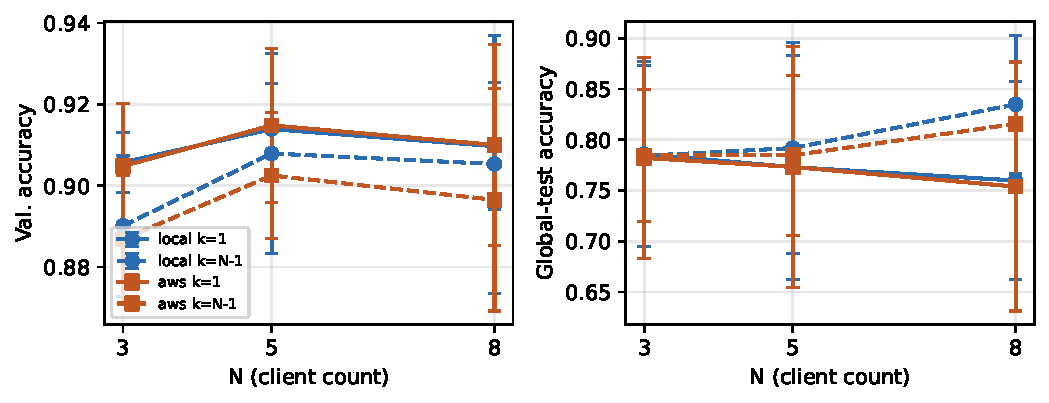
\includegraphics[width=\linewidth]{accuracy_vs_n}
  \caption{Accuratezza di validazione (sinistra) e sul global test set
  (destra) al variare di $N$, per $k=1$ e $k=N-1$, locale vs.\ AWS.}
  \label{fig:accuracy_vs_n}
\end{figure}

\subsection{Overhead di comunicazione}
Ogni messaggio push trasporta l'intero \texttt{state\_dict} del modello. Il traffico totale
stimato (Fig.~\ref{fig:communication}) cresce con $N$ e, soprattutto, con
$k$: a $N=8$, passare da $k=1$ a $k=N-1$ porta il numero di messaggi
scambiati da 295 a 1863 in locale e da 320 a 1303 su AWS. Questo è il costo diretto, e prevedibile, della scelta di $k$:
l'aumento di accuratezza global-test osservato con $k$ alto
(Fig.~\ref{fig:accuracy_vs_n}) va quindi letto come un compromesso esplicito
comunicazione/qualità.

\begin{figure}[t]
  \centering
  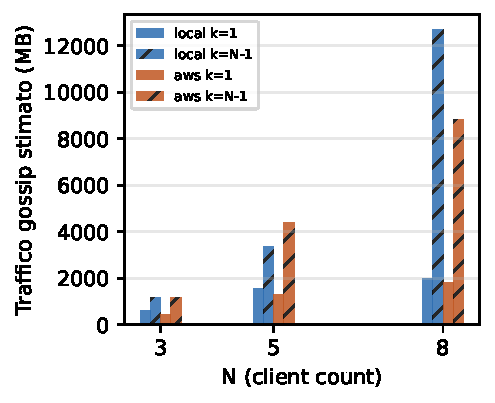
\includegraphics[width=\linewidth]{communication_overhead}
  \caption{Traffico totale stimato (messaggi $\times$ 6,82\,MB) per
  configurazione.}
  \label{fig:communication}
\end{figure}

\subsection{Dove viene speso il tempo}
La Fig.~\ref{fig:phase_timing} scompone la durata media di un round nelle tre
fasi definite in Sezione~\ref{sec:details}B. In locale la Fase A  dura 5--13\,s, la Fase B  0,3--6,9\,s in
funzione di $H$, la Fase C resta sotto i 340\,ms anche con
$k=N-1$. Su AWS la Fase A si stabilizza attorno a 109--126\,s
indipendentemente da $N$ e da $H$ — un valore pressoché costante compatibile
con un collo di bottiglia sul throughput di inferenza delle istanze
\texttt{t3.small} piuttosto che con un effetto del
workload. La Fase C, invece, resta nello stesso ordine di grandezza del caso
locale (60--227\,ms) anche attraverso rete reale tra istanze EC2 separate:
l'overhead di comunicazione del protocollo di push non è la causa del
rallentamento osservato su AWS.

\begin{figure}[t]
  \centering
  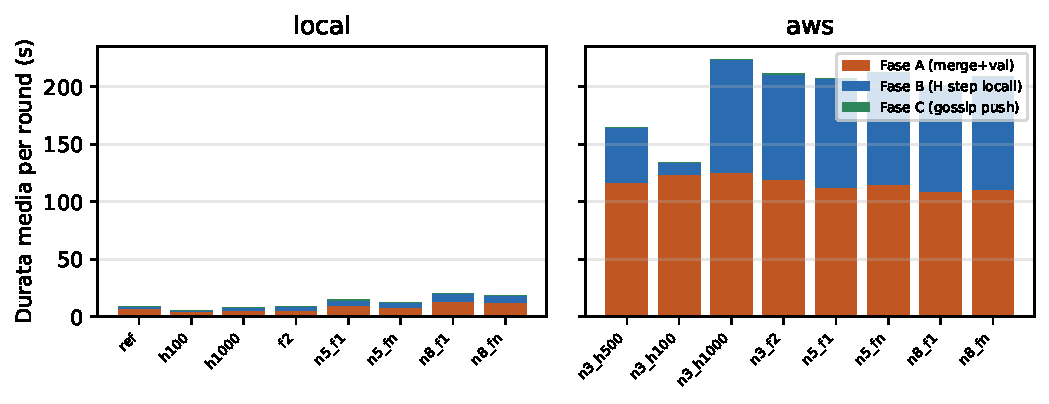
\includegraphics[width=\linewidth]{phase_timing}
  \caption{Durata media delle fasi A, B, C per round, locale vs.\ AWS.}
  \label{fig:phase_timing}
\end{figure}

\subsection{Locale vs.\ AWS multi-istanza}
Per le 8 configurazioni condivise dai due ambienti, la
Fig.~\ref{fig:local_vs_aws} confronta wall-clock di sistema e spread
global-test. Il wall-clock su AWS è 8--32$\times$ superiore a quello locale
per la stessa configurazione (dominato dalla Fase A, come discusso sopra).
Lo spread global-test resta invece in una banda solo in parte sovrapposta tra
i due ambienti: 12--30\% su AWS contro 15--25\% in locale — un intervallo
più ampio lato AWS, trainato dal 30,1\% di \texttt{n8\_f1} (il valore più
alto misurato in tutta la campagna) e dal 12,0\% di \texttt{n3\_f2} (il più
basso). Non emerge quindi un vantaggio sistematico di un ambiente
sull'altro sulla qualità della convergenza funzionale, ma la dispersione tra
configurazioni è più marcata su AWS in questa campagna.

\begin{figure}[t]
  \centering
  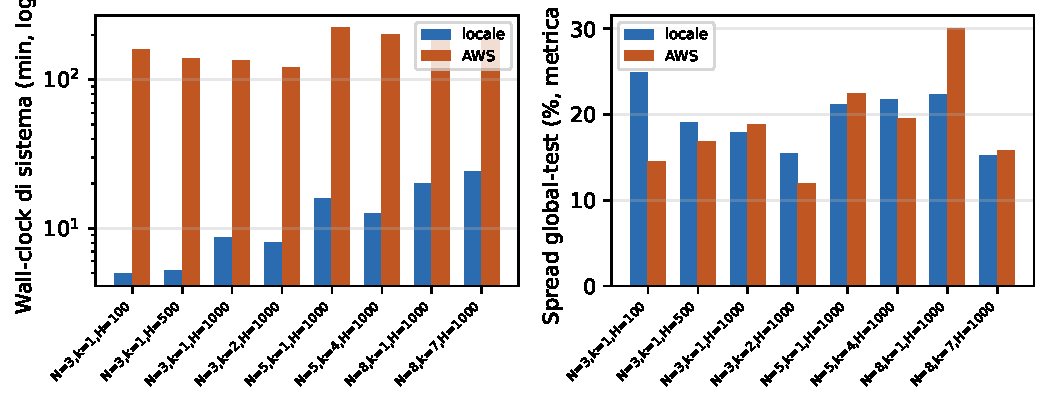
\includegraphics[width=\linewidth]{local_vs_aws}
  \caption{Wall-clock di sistema (scala log) e spread di accuratezza
  global-test, per le 8 configurazioni condivise da locale e AWS.}
  \label{fig:local_vs_aws}
\end{figure}

\subsection{Analisi per classe: matrice di confusione (campagna AWS)}
La campagna AWS qui riportata calcola, oltre ad accuratezza aggregata e
spread, anche precision/recall/F1 macro (media semplice tra le 62 classi,
non pesata per il numero di campioni di ciascuna — a differenza
dell'accuratezza aggregata) e la matrice di confusione completa
sul global test set per ciascuna configurazione. La
Tabella~\ref{tab:macro} riporta le metriche macro medie tra worker, con lo
stesso criterio [B] (checkpoint a minima validation loss) usato per
l'accuratezza in Tabella~\ref{tab:master}.

\begin{table*}[t]
  \centering
  \caption{Metriche macro sul global test set, media tra worker, per le 8 configurazioni AWS (criterio [B]).}
  \label{tab:macro}
  \scriptsize
  \begin{tabular}{lrrrrrr}
    \toprule
    \textbf{Config} & $N$ & $k$ & \textbf{Macro-precision} & \textbf{Macro-recall} & \textbf{Macro-F1} & \textbf{Spread F1} \\
    \midrule
    n3\_h500  & 3 & 1 & 0.750 & 0.710 & 0.685 & 11.2\% \\
    n3\_h100  & 3 & 1 & 0.719 & 0.678 & 0.643 & 7.2\%  \\
    n3\_h1000 & 3 & 1 & 0.764 & 0.730 & 0.698 & 13.7\% \\
    n3\_f2    & 3 & 2 & 0.757 & 0.747 & 0.715 & 10.0\% \\
    n5\_f1    & 5 & 1 & 0.772 & 0.732 & 0.704 & 20.1\% \\
    n5\_fn    & 5 & 4 & 0.775 & 0.742 & 0.714 & 15.5\% \\
    n8\_f1    & 8 & 1 & 0.758 & 0.708 & 0.679 & 28.6\% \\
    n8\_fn    & 8 & 7 & 0.786 & 0.752 & 0.742 & 13.2\% \\
    \bottomrule
  \end{tabular}
\end{table*}

Il macro-F1 segue lo stesso ordinamento qualitativo dell'accuratezza
aggregata (\texttt{n8\_fn} migliore, \texttt{n8\_f1} e \texttt{n3\_h100}
peggiori) ma è sistematicamente più basso di essa (0,64--0,74 contro
0,74--0,82 di accuratezza): la differenza è attesa, perché l'accuratezza
aggregata pesa ogni campione allo stesso modo mentre il macro-F1 pesa ogni
\emph{classe} allo stesso modo — su FEMNIST, dove alcune classi hanno
migliaia di campioni e altre poche centinaia (Sezione~\ref{sec:background}C),
un'accuratezza aggregata alta può convivere con prestazioni scarse sulle
classi rare, ed è esattamente ciò che il macro-F1 rivela.

Sommando le matrici di confusione dei worker di ciascuna run, lo schema degli
errori è pressoché identico nelle 8 configurazioni: le stesse tre coppie di
caratteri dominano gli errori in tutti e 8 i run — \texttt{l}$\to$\texttt{1}
(56--74\% delle occorrenze della vera classe \texttt{l}),
\texttt{O}$\to$\texttt{0} (52--73\%) e \texttt{I}$\to$\texttt{1}
(44--62\%) — e le classi con recall più basso sono, senza eccezioni tra le
8 run, \texttt{o} (lettera minuscola), \texttt{l} e \texttt{q}; \texttt{I}
è tra le peggiori in 7 delle 8 configurazioni (l'eccezione è
\texttt{n8\_fn}, dove al suo posto compare \texttt{p}).
Il caso più estremo è la lettera minuscola \texttt{o}: recall tra lo 0\% e
lo 0,9\% in tutte le configurazioni, con il 94\% circa dei suoi campioni
classificati come cifra \texttt{0} (dato dalla run \texttt{n8\_fn}, la più
accurata della campagna). In pratica il modello collassa la terna
\texttt{0}/\texttt{O}/\texttt{o} quasi interamente sulla cifra e la terna
\texttt{1}/\texttt{l}/\texttt{I} quasi interamente sulla cifra \texttt{1} —
una conferma empirica diretta dell'ambiguità visiva già anticipata come
motivazione del label smoothing (Sezione~\ref{sec:details}E): sono
esattamente le stesse coppie di caratteri citate lì come esempio. La
consistenza dello schema attraverso tutte le configurazioni suggerisce che
non sia un effetto della topologia di comunicazione o della scala $N$, ma
un limite del compito stesso (ambiguità geometrica intrinseca tra alcune
classi di FEMNIST) che nessuna delle configurazioni testate risolve.

\section{Discussion}
\label{sec:discussion}

\subsection{Il grado di gossip come compromesso esplicito}
A $N$ fissato, un $k$ più alto porta più aggiornamenti per round e, nella
maggior parte delle configurazioni testate ($N=5$ e $N=8$, sia in locale sia
su AWS), un'accuratezza global-test più alta a parità di $H$ — coerente con
l'attesa che un mixing più denso tra i pesi dei worker riduca la divergenza
verso soluzioni funzionalmente diverse. A $N=3$ l'effetto è invece piatto o
leggermente negativo in entrambi gli ambienti: con solo due vicini possibili,
passare da $k=1$ a $k=2$ non introduce una differenza qualitativa nella
topologia di comunicazione, e il rumore tra worker (tre soli campioni per
configurazione) è dello stesso ordine di grandezza dell'effetto misurato.
Questo guadagno non è gratuito: il traffico cresce nella stessa proporzione
di $k$ (Sez.~\ref{sec:results}C), per cui la scelta di $k$ va sempre motivata
rispetto al budget di banda disponibile, non solo rispetto all'accuratezza
target.

\subsection{Comunicazione non è il collo di bottiglia}
Un risultato rilevante ai fini dell'efficienza di comunicazione è che, anche
su rete reale tra istanze EC2 fisicamente separate, la Fase C resta
un'operazione dell'ordine delle centinaia di millisecondi, mentre il
rallentamento di oltre un ordine di grandezza osservato su AWS rispetto al
locale è concentrato nella Fase A (Sez.~\ref{sec:results}D), compatibile con
un limite di CPU burstable delle istanze \texttt{t3.small} piuttosto che con
un costo di rete. Questo supporta la scelta progettuale di comunicare
snapshot completi del modello a bassa frequenza ($H$ passi locali tra un
invio e l'altro) invece di aggiornamenti più frequenti e piccoli: nel regime
qui testato il costo di calcolo locale domina comunque quello di
comunicazione, per cui ridurre ulteriormente la frequenza di gossip non
avrebbe portato benefici proporzionali sul tempo totale.

\subsection{Nota metodologica sulla metrica di convergenza funzionale}
Lo strumento di analisi usato calcola lo spread di accuratezza sul global
test set in due varianti: al round finale di ciascun worker (quella usata
nella documentazione tecnica interna del progetto, ma esplicitamente
etichettata come riferimento rumoroso) e al round del checkpoint migliore di
ciascun worker (la metrica dichiarata primaria). Le due varianti possono
discordare sensibilmente per lo stesso run: per due delle configurazioni a
$N=3$, la variante \emph{riferimento} suggeriva uno spread contenuto
(4,5--4,8\%), mentre la metrica primaria mostra per le stesse run uno spread
del 19,5--21,1\%, in linea con tutte le altre 14 configurazioni. In questo
lavoro si è scelto di riportare sempre e solo la metrica primaria
(Tabella~\ref{tab:master}), proprio per evitare di presentare come
rappresentativo un valore isolato e più favorevole ottenuto con la metrica
esplicitamente definita come rumorosa.

\subsection{Limitazioni}
\begin{itemize}
  \item \textbf{Convergenza funzionale incompleta.} In nessuna delle 16
        configurazioni lo spread di accuratezza sul global test set scende
        sotto il 14\%: il protocollo gossip riduce ma non elimina la
        divergenza tra i modelli dei worker nel budget di round testato. I
        dati grezzi mostrano inoltre oscillazioni marcate round-su-round per
        singoli worker (in un caso, l'accuratezza global-test di un worker
        scende di 28 punti percentuali tra il proprio checkpoint migliore e
        il round finale), sintomo di instabilità subito dopo un merge FedAvg
        con vicini divergenti.
  \item \textbf{Singola replica per configurazione.} Nessun run è stato
        ripetuto con seed diverso: la deviazione standard riportata è
        \emph{tra worker} dello stesso run, non \emph{tra run} della stessa
        configurazione, e non permette di separare con certezza l'effetto di
        un iperparametro dalla variabilità intrinseca del processo.
  \item \textbf{Confondimento in una configurazione AWS.} Il run
        \texttt{n8\_fn} su AWS usa \texttt{early\_stopping\_patience=7}
        anziché 10 come tutti gli altri 15 run, per un errore di
        configurazione: il confronto diretto di questa configurazione con le
        altre a $N=8$ va quindi interpretato con cautela.
  \item \textbf{Peer effettivamente contattati sotto il target.} Il numero
        medio di vicini contattati da un worker può scendere sotto il valore
        di $k$ configurato quando altri worker terminano in anticipo
        (early stopping locale) e si deregistrano, riducendo il pool di peer
        disponibili — un effetto emergente dell'asincronia tra worker, non
        un difetto del meccanismo di selezione.
  \item \textbf{Assenza di heartbeat.} Il sistema rileva un peer caduto solo
        al primo fallimento di invio verso di esso; un crash non pulito
        (SIGKILL, OOM) lascia una entry non valida nel discovery server fino
        a quel momento, senza un meccanismo di TTL attivo. Questa è una
        scelta deliberata, non una svista: un heartbeat periodico verso il
        discovery server introdurrebbe traffico di coordinamento che cresce
        con $N$ e con la frequenza del battito, in diretto contrasto con
        l'obiettivo di traffico ridotto che guida le altre scelte
        protocollari di questo lavoro (cache dei peer, k-push a singolo hop);
        il costo è stato giudicato non giustificato per un caso d'uso — il
        crash non pulito — fuori dal perimetro sperimentale di questo lavoro.
  \item \textbf{Statistiche di Batch Normalization non aggregate.} Solo i
        parametri appresi (scala e bias) sono mediati da FedAvg; le
        statistiche correnti di media e varianza restano locali a ciascun
        worker, una scelta nota in letteratura per introdurre un
        disallineamento tra i client dopo l'aggregazione~\cite{li2021fedbn}.
\end{itemize}

\subsection{Confronto con la letteratura}
FedAvg centralizzato su FEMNIST è tipicamente riportato in letteratura
attorno al 77--80\% di accuratezza di test~\cite{li2020fedprox}. Le
configurazioni qui testate raggiungono un'accuratezza di validazione più alta
(87--91\%) ma un'accuratezza global-test più bassa (75--85\%): il confronto
diretto non è però del tutto omogeneo, poiché la validazione qui misurata
avviene su campioni tenuti da parte dagli stessi scrittori visti in training,
mentre il global test set contiene scrittori mai visti da nessun worker — un
compito di generalizzazione più severo, e più vicino allo scenario reale in
cui il modello deve funzionare su utenti non rappresentati nell'addestramento.

\section{Conclusions}
\label{sec:conclusions}

Questo lavoro ha presentato un sistema di Federated Learning decentralizzato
peer-to-peer, in cui FedAvg è eseguito tramite aggregazione online e gossip
$k$-push senza alcun aggregatore centrale per l'intera durata
dell'addestramento, e in cui la centralizzazione è confinata alla sola
discovery dei client. Il sistema è stato valutato su FEMNIST (LEAF) con
partizionamento non-i.i.d.\ per scrittore, in 16 configurazioni tra esecuzione
locale e deployment reale su AWS multi-istanza, raggiungendo un'accuratezza
di validazione dell'87--91\% e mostrando che, nel regime testato, il costo di
comunicazione del protocollo gossip resta trascurabile rispetto al costo del
calcolo locale, anche su rete reale. L'analisi ha inoltre evidenziato, in
modo trasparente, i limiti della convergenza funzionale ottenuta e le
condizioni sperimentali (singola replica, un confondimento di configurazione)
sotto cui i risultati vanno interpretati.

Sviluppi futuri naturali includono: l'introduzione di una strategia di
aggregazione alternativa a FedAvg (ad es.\ FedProx) per mitigare
esplicitamente il client drift osservato; una politica di $k$ adattivo che
tenga conto del numero di peer ancora attivi; e la ripetizione delle
configurazioni con seed multipli per quantificare rigorosamente la varianza
run-to-run qui non misurata.

Due estensioni indirizzerebbero più a fondo la tolleranza ai guasti, oggi
solo parzialmente coperta (Sezione~\ref{sec:discussion}D). Per il rientro
dopo un crash, il checkpoint locale già salvato a ogni miglioramento della
validation loss potrebbe essere esteso con il numero di round: un worker
riavviato si ri-registrerebbe con lo stesso identificativo e riprenderebbe
da quel checkpoint invece che da zero, mentre il controllo di staleness già
presente assorbirebbe naturalmente il disallineamento di round rispetto agli
altri worker. Per l'ingresso live di un client nuovo, il discovery server
accetta già registrazioni in qualunque momento, ma oggi il nuovo worker
partirebbe da pesi casuali; aggiungendo al protocollo gRPC una RPC di
\emph{pull} accanto all'attuale \emph{push}, un worker entrante potrebbe
richiedere una sola volta i pesi correnti a un peer attivo come
inizializzazione, per poi partecipare ai round successivi come tutti gli
altri.


\bibliographystyle{IEEEtran}
\bibliography{references}

\end{document}
